%!TEX root =  main.tex
\section{Performance evaluation}
\label{sec:experiments}

In this section, we report results from two benchmarks: TPC-C and
\appname{} social networking service described in the previous section.
Our experiments show that \dynastar{} is able to rapidly adapt to changing 
workloads, while achieving throughputs and latencies far better than the existing
state-of-the-art approaches to state machine replication partitioning.


\subsection{Experimental environment}
\label{sec:evaluation:setup}

We conducted all experiments on Amazon EC2 T2 large instances (nodes). Each node has 8 GB of RAM, 
two virtual cores and is equipped with an Amazon EBS standard SSD with a maximal bandwidth 10000 IOPS.
All nodes ran Ubuntu Server 16.04 LTS 64 and had the OpenJDK Runtime Environment~8 with the
\mbox{64-Bit} Server VM (build 25.45-b02). In all experiments, the oracle 
had the same resources as every other partition: 2 replicas and 3 Paxos acceptors 
(in total five nodes per partition).


% \subsection{Methodology and goals}
% \label{sec:evaluation:methodology}

% %In order to show the scalability of our approach we tested the performance as the 
% %number of partitions increases, and performance as the size and complexity of the graph grows.
% The experiments seek to answer the following questions:
% \begin{itemize}
% \item \emph{What is the impact of repartitioning on a real dataset?}
% \item \emph{How does partitioning affect performance when the workload grows with the number of partitions and when the workload has constant size?}
% \item \emph{How does \dynastar performance compare to other approaches?} 
% \item \emph{How does \dynastar perform under dynamic workloads?}
% \item \emph{What is the performance of the oracle?}
% \end{itemize}

%\paragraph*{Performance metrics.}
%%
%The latency was measured as the end-to-end time between issuing the
%command, and receiving the response.  Throughput was measured as the
%number of posts/second or transactions/second that the clients were able to send.

\subsection{TPC-C benchmark}
\label{sec:evaluation:tpc-c}

In the experiments in this section, we deploy as many partitions as the number of warehouses.

%\paragraph*{The impact of graph repartitioning}
\subsubsection{The impact of graph repartitioning}
In order to assess the impact of state partitioning on performance, we ran the TPC-C benchmark on an 
un-partitioned database.  Figure ~\ref{fig:tpcc_repartitioning} 
shows the performance of \dynastar with 8 warehouses and 8 partitions.
At the first part of the experiment, all the variables are randomly distributed across all partitions.
As a result, almost every transaction accesses all partitions. Thus every transaction 
required coordination between partitions, and objects were constantly moving back and forth. 
%In addition, transactions from different clients were blocked by the others, 
%made the time it took for executing one transaction remarkably high.
This can be observed in the first 50 seconds of the experiment depicted in Figure 
~\ref{fig:tpcc_repartitioning}: low throughput (i.e., a few transactions executed per second), 
high latency (i.e., several seconds), and a high percentage of cross-partition transactions.


%In addition to that, when a partition takes part in an execution of a transaction, 
%if another command access variables that are being accesses by the ongoing command will 
% be blocked until the previous command finish

After 50 seconds, the oracle computed a new partitioning based on previously executed transactions 
and instructed the partitions to apply the new partitioning.
When the partitions delivered the partitioning request, they exchanged objects to achieve the new partitioning.
% During this process, servers didn't execute any other transactions, thus the throughput decreased 
% to 0, and the average latency was not applicable. 
It takes about 10 seconds for partitions to reach the new partitioning.
However, during the repartitioning, servers continue to execute transactions.
After the state is relocated, most objects involved in a transaction
can be found in a local partition, which considerably increases performance and reduces latency. 

\begin{figure}[ht!]
  \centering
    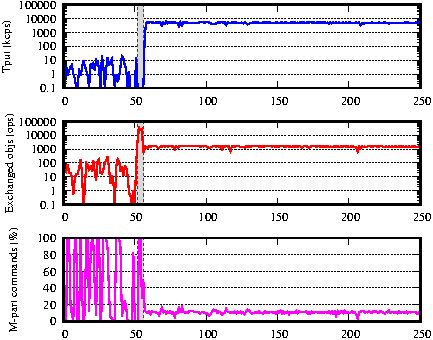
\includegraphics[width=0.8\columnwidth]{figures/experiments/tpcc-detail-dynastar}
  \caption{Repartitioning in \dynastar; throughput (top), objects exchanged between partitions (middle), 
  and percentage of multi-partition commands (bottom).}
  \label{fig:tpcc_repartitioning}
\end{figure}

\subsubsection{Scalability}
In order to show how \dynastar scales out, we varied the number of partitions from 1 to 128 partitions. 
%We also added warehouses while adding partitions to demonstrate using 
%\dynastar to grow an application by adding more hardware. 
We used sufficient clients to  saturate the throughput of the system in each experiment. 
Figure ~\ref{fig:tpcc_scaling} shows the peak throughput of \dynastar and S-SMR* as we vary the 
number of partitions. 
Notice that we increase the state size as we add partitions (i.e., there is one warehouse per partition).
The result shows that \dynastar is capable of applying
a partitioning scheme that leads to scalable performance.

\begin{figure}[ht!]
  \centering
    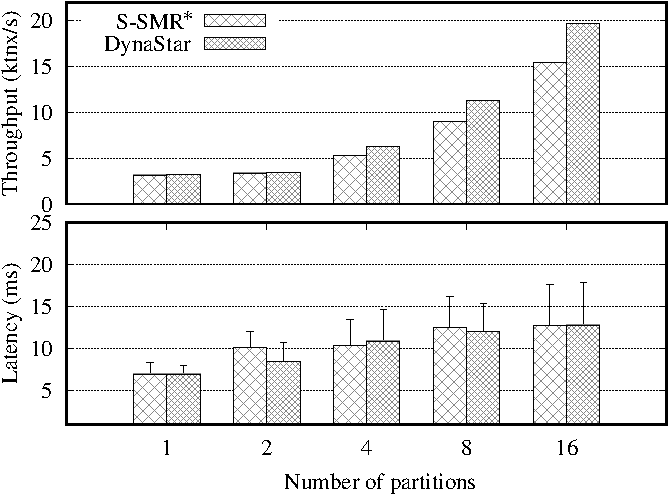
\includegraphics[width=0.8\columnwidth]{figures/experiments/tpcc-scaling-tp-lat.pdf}
  \caption{Performance scalability with TPC-C. Throughput (in thousands of transactions per second, ktps) and latency for $\approx$75\% peak throughput in milliseconds (bars show average, whiskers show 95-th percentile).}
  \label{fig:tpcc_scaling}
\end{figure}

\subsection{Social network}

%\paragraph*{Workloads.}
We used the Higgs Twitter dataset~\cite{snapnets} as the social graph in the experiments. 
The graph is a subset of the Twitter network that was built based on the monitoring of the spreading
of news on Twitter after the discovery of a new particle with the features of the elusive 
Higgs boson on 4th July 2012. The dataset consists of 456631 nodes and more than 14 million edges.
%Graphs with 0\% of edge-cuts have \emph{strong locality}.

We evaluate the performance of \dynastar and other techniques. With S-SMR*, we used
METIS to partition the data in advance. Thus, S-SMR* started with an optimized partitioning. \dynastar started with
random location of the objects. Each client issues a sequence of commands.  
For each command, the client selects a random node as the active user with Zipfian access pattern ($\rho$ = 0.95).
We focused on two types of workloads: timeline only commands and mix commands (85\% timeline and 15\% post). 
Each client operates in a closed loop, that is, the client issues a command and then waits from the response to submit the next command.

% \paragraph*{Command generation.}
% %

%\begin{figure}[ht]
%  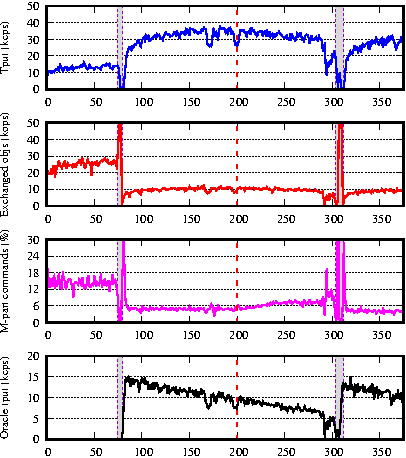
\includegraphics[width=0.95\columnwidth]{figures/experiments/chirper-celeb-dynastar}
%  \caption{Dynamic partitioning with DynaStar.}
%  \label{fig:4p1p_varying_partition_size}
%\end{figure}
%
\begin{figure}[ht]
 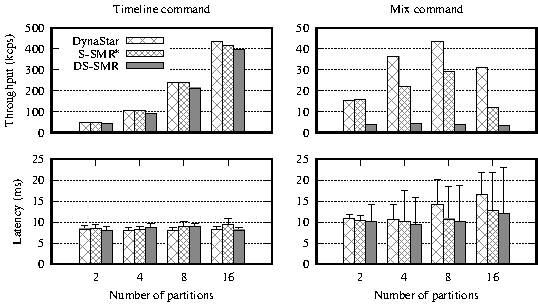
\includegraphics[width=0.99\columnwidth]{figures/experiments/chirper-compare-full}
 \caption{Performance of social network service. Throughput (in thousands of commands per second, kcps) and latency for different partitions. 
  Latency for $\approx$75\% peak throughput in milliseconds (bars show average, whiskers show 95-th percentile).}
  \label{fig:socialscalability}
\end{figure}

% \begin{figure*}[h]
%   \centering
%   \begin{subfigure}{0.95\columnwidth}
%     \begin{subfigure}{.45\columnwidth}
%       \centering
%       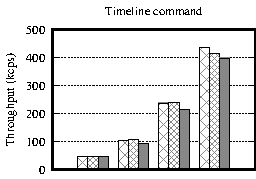
\includegraphics[width=\columnwidth]{./figures/experiments/chirper-compare-timeline-tp.pdf}
%     \end{subfigure}
%     % \hfill %%
%     \begin{subfigure}{.45\columnwidth}
%       \centering
%       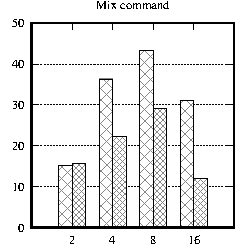
\includegraphics[width=\columnwidth]{./figures/experiments/chirper-compare-mix-tp.pdf}
%     \end{subfigure}
%   \end{subfigure}
%   \vfill %%
%   \begin{subfigure}{0.95\columnwidth}
%     \begin{subfigure}{.45\columnwidth}
%       \centering
%       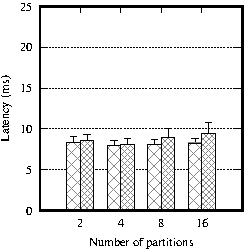
\includegraphics[width=\columnwidth]{./figures/experiments/chirper-compare-timeline-lat.pdf}
%     \end{subfigure}
%     \hfill %%
%     \begin{subfigure}{.45\columnwidth}
%       \centering
%       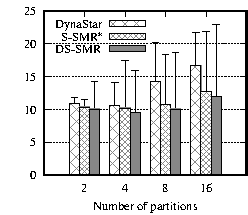
\includegraphics[width=\columnwidth]{./figures/experiments/chirper-compare-mix-lat.pdf}
%     \end{subfigure}
%   \end{subfigure}
%   \caption{Throughput and latency for different partition numbers. 
%   Throughput is in thousands of commands per second (kcps). 
%   Latency for $\approx$75\% peak throughput is in milliseconds (bars show average, whiskers show 95-th percentile).}
%   \label{fig:socialscalability}
% \end{figure*}


\subsubsection{\dynastar vs. other techniques}
\label{sec:evaluation:results}

Figure~\ref{fig:socialscalability} shows the peak throughput and latency for approximately 75\% of peak throughput
 (average and 95-th percentile) of the evaluated techniques as we vary the number of 
 partitions of the fixed graph for the social networks.

In the experiment with timeline commands, all three techniques perform similarly. This happens because no moves occur in
\dynastar or \dssmr{}, and no synchronization among partitions is necessary for S-SMR* in this case. 
Consequently, all three schemes scale remarkably well, and
the difference in throughput between each technique is due to the implementation of each one.
%Although \dynastar and DS-SMR have comparable performance, they differ in an important way. 
%As shown in Figure~\ref{fig:motivation} (top left graph) for 4 partitions, \dynastar converges 
%to maximum throughput after 20 seconds from the beginning of the execution, while it takes 
%DS-SMR (decentralized dynamic scheme) about 80 seconds to converge.
%This means that \dynastar can react to workload changes more rapidly than DS-SMR.


% With social networks with edge cut percentage greater than zero \dssmr\ performance decreases significantly.  
% This happens because in such cases, objects in \dssmr\ are constantly being moved back and forth between partitions 
% without converging to a stable configuration.
% %(see also Figure~\ref{fig:motivation}, graph on the bottom right, for 4 partitions). 
% In contrast, for \dynastar and \ssmr with an optimized partitioning, we see that the throughput scales with the number of partitions in experiments with up to 10\% of edge cuts. 
%With 10\% of edge cuts and above, the overhead from moves (in \dynastar) and cross-partition commands (in S-SMR) outweighs the gains from additional partitions.

In the experiment with the mix workload, we see that \dssmr{} performance decreases significantly.
This happens because in such cases, objects in \dssmr{} are constantly moving back and forth 
between partitions without converging to a stable configuration.
In contrast, for \dynastar and S-SMR*, the throughput scales with 
the number of partitions in experiments with up to 8 partitions. 
Increasing the number of partitions to 16 with the fixed graph reveals a tradeoff:
On the one hand, additional partitions should improve performance as there are more resources to execute commands.
On the other hand, the number of edge cuts increases with the number of partitions, which hurts performance 
as there are additional operations involving multiple partitions.

Notice that only post operations are subject to this tradeoff since they may involve multiple partitions.
The most common operation in social networks is the request to read a user timeline. This is a single-partition
command in our application and as a consequence it scales linearly with the number of partitions.

% Figure~\ref{fig:socialcdf} shows the cumulative distribution functions (CDFs) of latency for the mix workload of \dynastar and S-SMR* on different configurations. The results suggest that S-SMR* achieves lower latency than \dynastar for 80\% of the load. This is expected, as for multi-partition commands, partitions in \dynastar have to send additional data to return objects to their original location after command execution . 


% \paragraph*{The ideal number of partitions.}
% \label{sec:evaluation:results}

% While in the previous section we considered executions with a fixed percentage of edge cuts.
% %, as we increased the number of partitions 
% %(by adjusting the social graph clustering coefficient),
% We now consider a fixed social network graph and vary the number of partitions.
% Increasing the number of partitions with a fixed graph introduces a tradeoff.
% On the one hand, additional partitions improve performance as there are more resources to execute posts.
% On the other hand, the number of edge cuts increases with the number of partitions, which hurts performance as there are additional operations involving multiple partitions.
% We evaluate the performance of \dynastar, \dssmr\ and \ssmr with an optimized partitioning.% when subject to this tradeoff. 

% Figure~\ref{fig:4p1p_varying_partition_size} shows that \dynastar and optimized \ssmr throughput scale up to ten partitions, after which performance decreases. \dssmr\ throughput decreases gradually as we increase partitions, since the chance that objects are spread between partitions also increases.
% % For each configuration, we computed the percentage of edge cuts and found that for 2, 3, 4, 6 and 8 partitions the percentages were respectively 
% % 0.13\%, 0.88, 1.06\%, 2.28\% and 2.67\%.
% Notice that only post operations are subject to this tradeoff since they may involve multiple partitions.
% The most common operation in social networks is the request to read a user timeline. This is a single-partition
% command in our application and as a consequence it scales linearly with the number of partitions.


\subsubsection{Performance under dynamic workloads}

Figure~\ref{fig:socialcelebrity} depicts the performance of \dynastar and S-SMR* with an evolving social network.  
We started the system with the original network from Higg dataset. After 200 seconds, we introduced a new celebrity user in the workload.
The celebrity user posted more frequently, and 
other users started following the celebrity. 

\begin{figure*}[h!]
  \centering
  \begin{subfigure}{.42\textwidth}
    \centering
    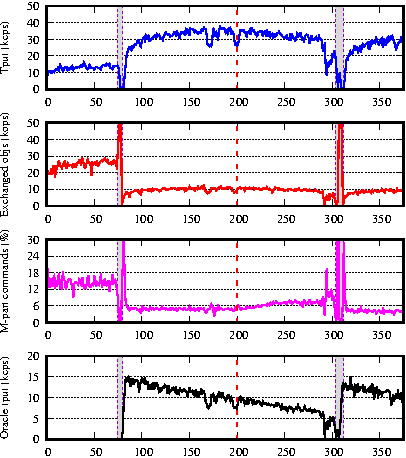
\includegraphics[width=\textwidth]{./figures/experiments/chirper-celeb-dynastar.pdf}
    \caption{}
  \end{subfigure}
  \begin{subfigure}{.42\textwidth}
    \centering
    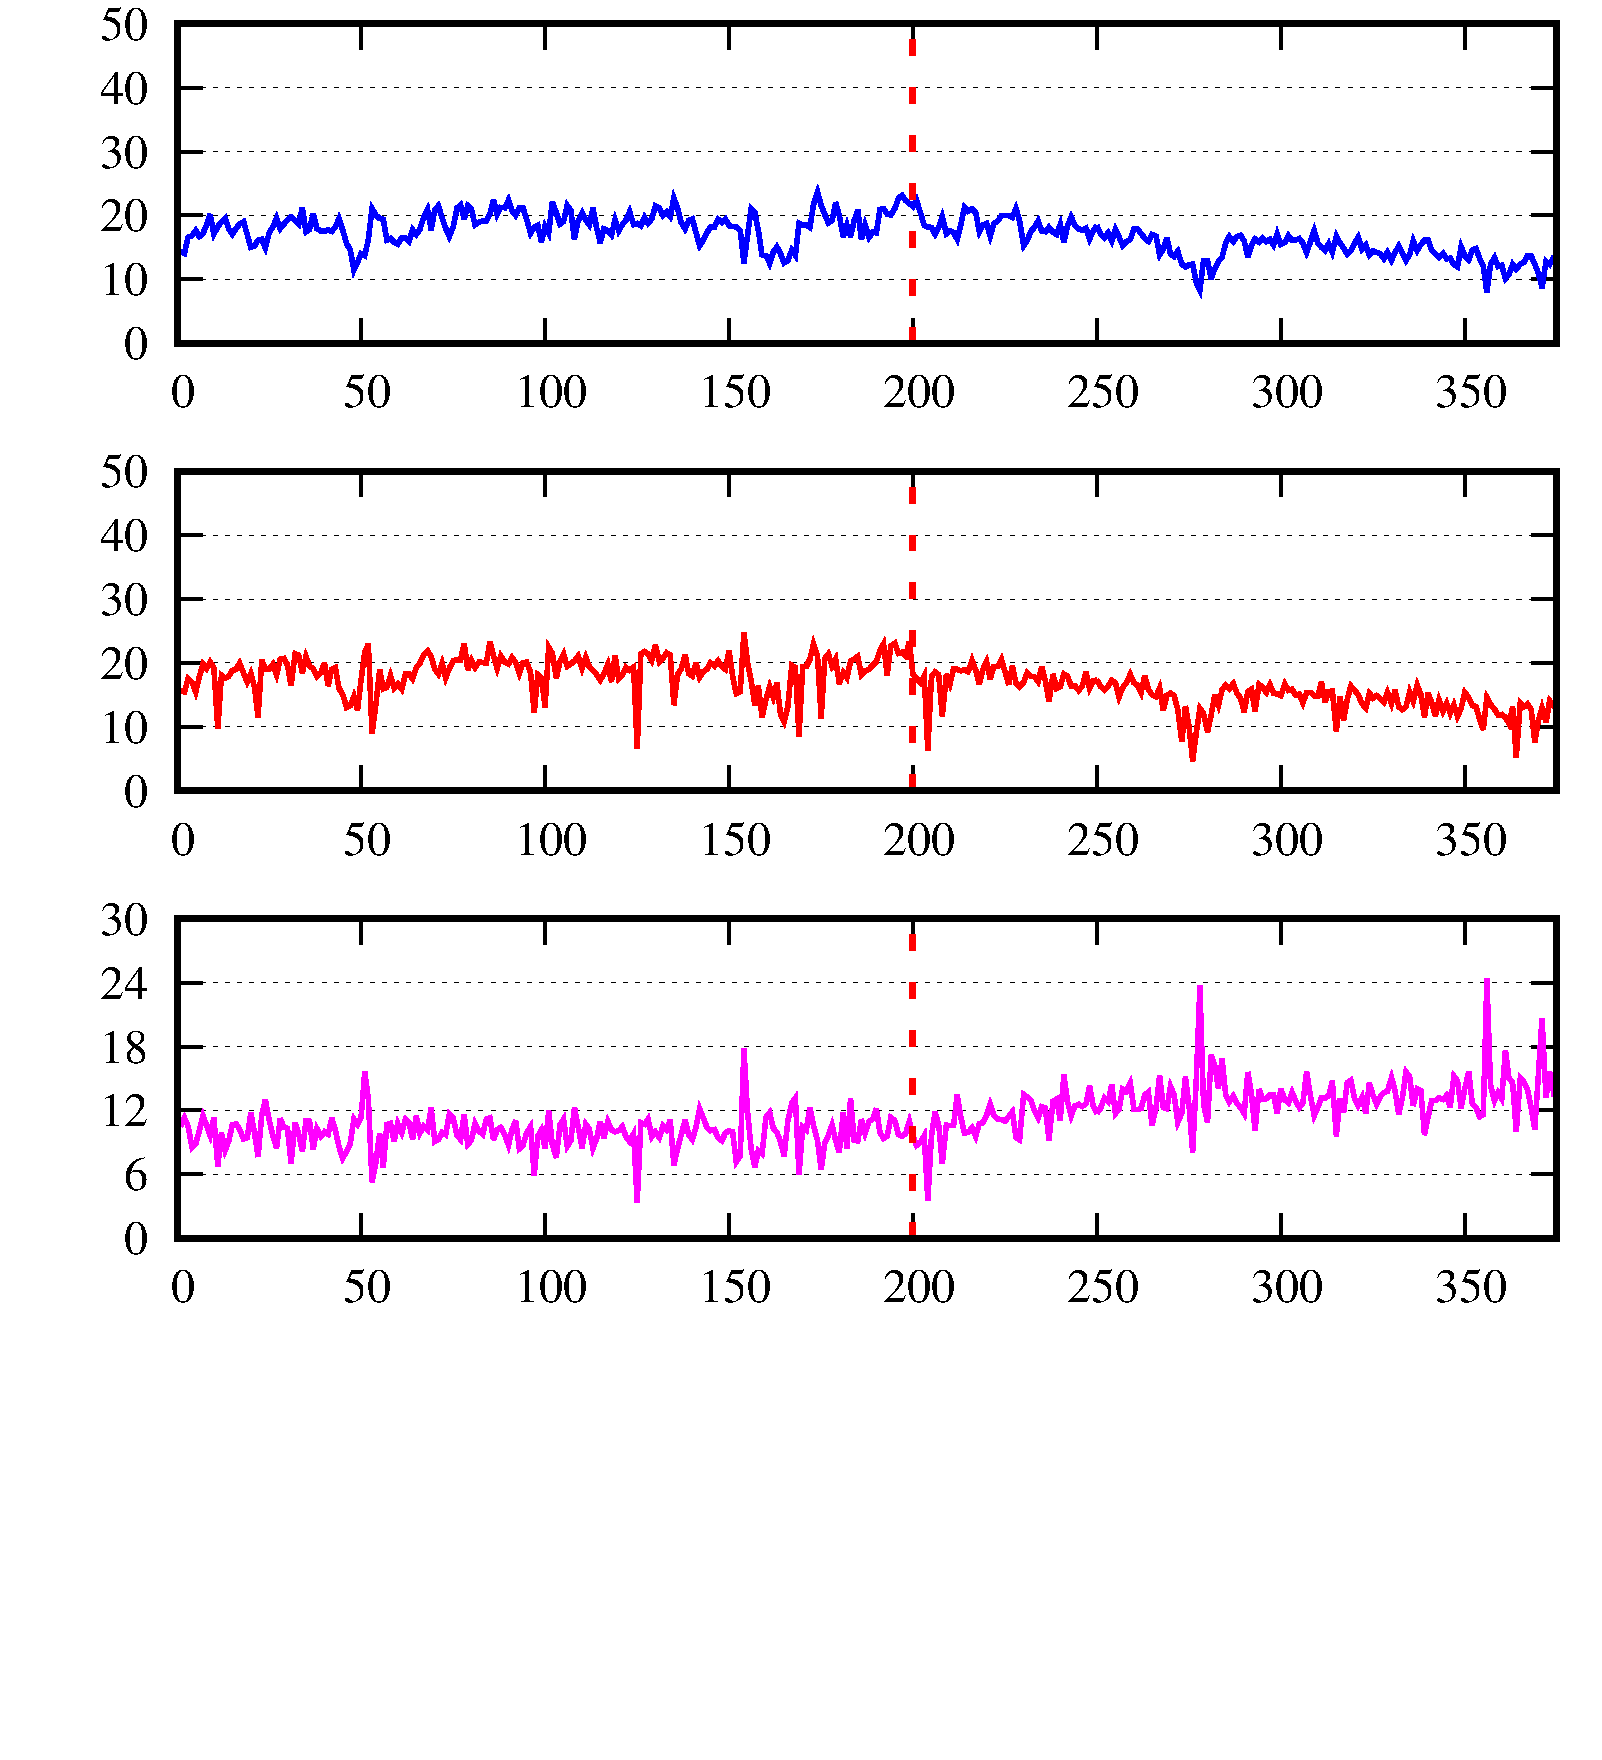
\includegraphics[width=\textwidth]{./figures/experiments/chirper-celeb-ssmr.pdf}
    \caption{}
  \end{subfigure}
  \caption{Repartitioning a dynamic workload with \dynastar~(a) and \ssmr* without repartitioning (b).}%
  \label{fig:socialcelebrity}
\end{figure*}

At the beginning of the experiment, \dynastar performance was not as good as S-SMR* (i.e., lower throughput, higher number of
percentage of multi-partition commands, and higher number of exchanged objects), because S-SMR* started with an optimized
partitioning, while \dynastar started with a random partitioning. 
After 50 seconds, \dynastar triggered the repartitioning process, which led to an optimized location of data. Repartitioning helped
reduce the percentage of multi-partition commands to 10\%, and thus increased the throughput. After the repartitioning, \dynastar outperforms S-SMR* with the optimized partitioning.
After 200 seconds, the network started to change its structure, as many users started to follow a celebrity, and created more edges
between nodes in the graph. Both \dynastar and S-SMR suffered from the change, as the rate of multi-partition command increased, and the throughput
decreased. However, when the repartitioning takes place in \dynastar, around 300 seconds into the execution, the previously user mapping
got a better location from the oracle, which adapted the changes. After the repartitioning, the objects are moved to a better partition, with a resulting increase in throughput.

% Table ~\ref{table:socialsnapshot} shows the throughput of each partition when the system reached the maximum throughput at the second of 180. Although the objects were evenly distributed among partitions, there was still a skew in the load of the system, e.g., partition 1 and 2 served more commands than the other partitions. This happened because of the skew in the access pattern: some users were more active and posted more than the others, thus the requests that sent to their servers are more than to other servers.

% \begin{table}[htp]
% \caption{Average load at partitions at peak throughput.}
% \begin{adjustbox}{max width=\columnwidth}
% \vspace{10mm}
% \begin{tabular}{|c|c|c|c|}
% \hline
% Partition & Tput & M-part commands per sec & Exchanged objects per sec \\ \hline
% 1         & 12766      & 887                      & 3907              \\ \hline
% 2         & 11790      & 643                      & 3036              \\ \hline
% 3         & 6775       & 440                      & 1503              \\ \hline
% 4         & 6458       & 400                      & 1490              \\ \hline
% \end{tabular}
% \label{table:socialsnapshot}
% \vspace{10mm}
% \end{adjustbox}
% \end{table}

\subsection{The performance of the oracle}

\dynastar  uses an oracle that maintains a global view of the workload graph. The oracle allows
\dynastar to make better choices about data movement, resulting in an overally
better throughput and lower latency. However, introducing a centralized
component in a distributed system is always a cause for some skepticism,
in case the component becomes a bottleneck, or a single point of failure. 
To cope with failures, the oracle is implemented as a replicated partition. 
The results in Figure~\ref{fig:socialcelebrity} suggest that the oracle would not become a bottleneck.
The number of queries processed to the oracle is zero at the 
beginning of the experiment, as the clients have cached the location of all objects.
After 80 seconds, the repartitioning was triggered, making all cached data on clients invalid.
Thus the throughput of queries at the oracle increases, when clients started asking for new location of variables.
However, the load diminishes rapidly and gradually reduce. This is because access to the oracle is necessary only
when clients have an invalid cache or when a repartition happens


% We conducted the experiment to evaluate if the \dynastar oracle is a bottleneck to
% system performance. The results show that the load on the oracle is
% low, suggesting that \dynastar scales well.


% The first experiment assesses the scalability of the METIS algorithm only.
% We measured the time to compute the partitioning solution, and
% the memory usage of the algorithms for increasingly large graphs. 
% The results, depicted in Figure~\ref{fig:metis_size_time}, show that METIS scales
% linearly in both memory and computation time on graphs of up to 10 million vertices.

% \begin{figure}[ht!]
%   \centering
%     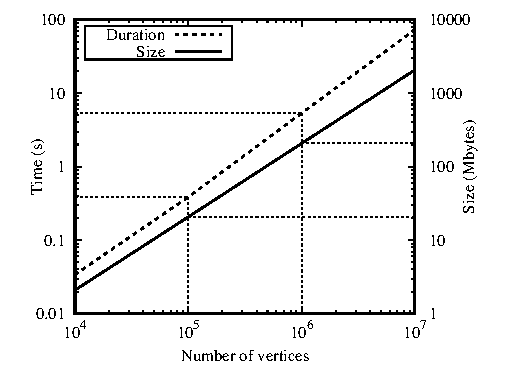
\includegraphics[width=\columnwidth]{figures/metis_size_time}
% 	\caption{METIS processor and memory usage.}
% 	\label{fig:metis_size_time}
% \end{figure}

% The experiment evaluates the oracle in terms of the number of queries sent to the oracle over
% time, for varying numbers of partitions. The experiment results was measured when the system was running stable, 
% and the clients had cache all requests.  The results are shown in
% Figure~\ref{fig:socialcelebrity}. The number of queries processed to the oracle is zero at the 
% beginning of the experiment, as the clients has cached the location of all objects.
% After 80 second, the repartitioning was triggers, made all the cache on clients invalid.
% Thus the throughput of queries at the oracle increases, when clients started asking for new location of variables.
% However, the load diminishes rapidly and gradually reduce to zero. This is because access to the oracle is necessary only
% when clients have an invalid cache or when a repartition happens. These experiments
% suggest that the oracle would not become a bottleneck.% for reasonably large
%deployments.

% \begin{figure}[ht]
% 	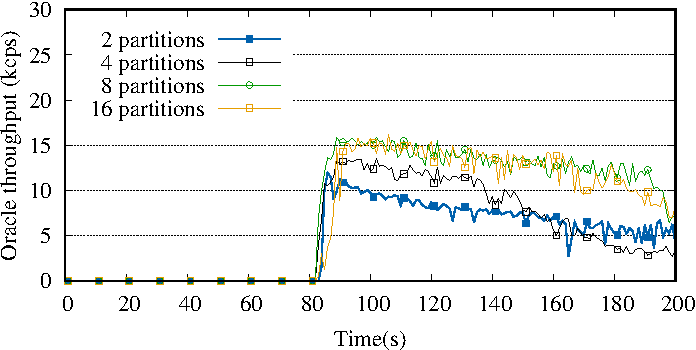
\includegraphics[width=\columnwidth]{figures/experiments/chirper-oracle-load.pdf}
%   \caption{Throughput at the oracle (social network).}
% 	\label{fig:cpu_oracle}
% \end{figure}

